% This work is licensed under
% http://creativecommon.org/licenses/by/3.0/
\section{Two patterns for implementing mobility}
\label{sec:sec3}

In this section we show that there are two completely different patterns
for implementing mobility.
They differ in where the change of attachment appears with respect to the
implementing layer,
in which algorithms and protocols of the implementing layer 
are involved in implementing mobility, and in which parts of the
shared state of the implementing layer are altered.
They also differ
in their detailed design
decisions, and in their cost, performance, and scalability issues.

Not only are these patterns non-overlapping, they also completely
cover all implementations of mobility, in the sense that each
implementation either follows one pattern or is clearly a composition
of the two patterns.

\subsection{Dynamic-routing mobility}
\label{sec:drm}

Figure~\ref{fig:drm} has two stages depicting the effect of mobility
on an inter-layer channel.
Recall that the channel is a {\it link}
in the state of the layer that uses it, and a {\it session} in the
state of the layer that implements it; its {\it higher endpoints}
are members in the user layer, while its {\it lower endpoints} are
members in
the implementing layer.

\begin{figure}
\centering
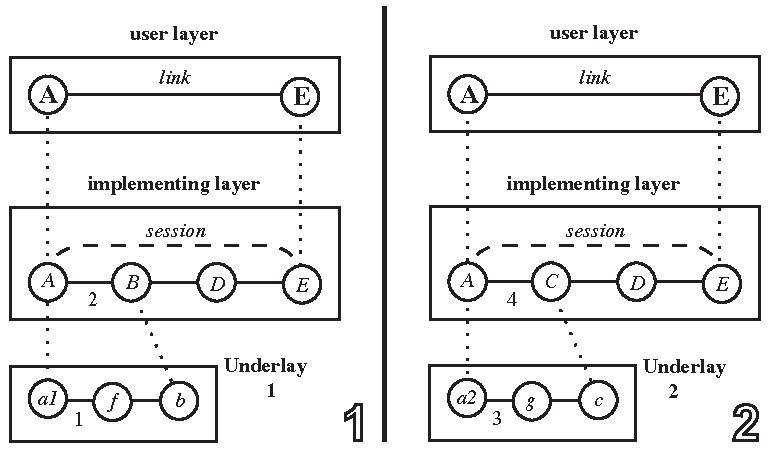
\includegraphics[scale=0.95]{figures/drm.pdf}
\caption{Two stages in an instance of dynamic-routing mobility.}
\label{fig:drm}
\end{figure}

The precise site of mobility here is the lower endpoint {\it A}.
In Stage 1 {\it A} is registered at {\it a1} in
Underlay 1.
{\it a1} and {\it A} are connected to the rest of their layers
through Links 1 and 2, respectively.  
Link 2 is implemented by Underlay 1.

Between Stage 1 and Stage 2
Link 1 stops working, possibly because the machine on which
{\it A} and {\it a1} reside has
been unplugged from a wired subnetwork, or
has moved out of range of a wireless subnetwork.
In a cascading sequence of events, 
Link 1 is destroyed,
Link 2 is destroyed, and the registration
of {\it A} at {\it a1} is destroyed. 
{\it A} is now disconnected from the rest of its layer.

Eventually the mobile machine may become plugged into another
wired subnetwork
or enter the range of another wireless subnetwork, as shown in Stage 2.
In a cascading sequence of events, member {\it a2} (which is
the mobile machine's member in the new Underlay 2)
connects to the rest of its layer through Link 3,
{\it A} becomes attached to new location {\it a2}, and new Link 4 is
created in the mobility layer and implemented by Underlay 2.
Note that {\it A} is now linked to {\it C} rather than {\it B};
this change is necessary because {\it C} is attached to Underlay 2 and
{\it B} is not.

Between Stages 1 and 2 there may be an interval during which {\it A}
has no connection with the rest of its layer.
There may also be an interval in which Stages 1 and 2 overlap, so
that {\it A} is temporarily attached to both underlays.

The hard problem to be solved in Figure~\ref{fig:drm} is that 
even after {\it A} is again reachable by other members of its layer
such as {\it D} and {\it E}, they do not know how to find it because
the routes to it are obsolete.
{\it Dynamic-routing mobility} relies on the routing algorithm of
the layer, which must learn about new links, recompute routes,
and update forwarding tables.
After this is accomplished, {\it D} will know that it can reach
{\it A} by forwarding to {\it C}.

There are three ways in which actual dynamic-routing
mobility can differ from the
example in Figure~\ref{fig:drm}.
Fortunately, none of them affect what the implementation has to do,
so none of them need be discussed separately.
First, the new attachment {\it a2} could be in the same layer as 
{\it a1}, rather than in a different layer.
Because {\it a1} and {\it a2} are different locations,
after the move {\it A} is probably linked to
a different member of its own layer, even though the new link is
implemented by the same lower layer as before.

Second, in Figure~\ref{fig:drm} the mobile member {\it A} has only
one attachment and one necessary link.
As shown in Figure~\ref{fig:scope}, members such as gateways have
multiple simultaneous attachments to different underlays.
Because each such attachment is necessary for the gateway's
purpose and supports its own link or links,
the mobility of each attachment is a separate problem to be solved.

Third, occasionally a layer implements sessions for the benefit of
its own members, rather than as a service to a higher user layer.
In this case there is no {\bf A} or {\bf E}, and the beneficiaries of
the mobility implementation are {\it A} and {\it E}.

A {\it router} is a member of a layer that receives and forwards messages
not destined for itself, whether it sends and receives messages on its
own behalf or not.
A {\it forwarding table} is a distributed copy of some of the
{\it routes} state component of a layer.
Implementations of dynamic-routing mobility incur four kinds of
resource cost:
\begin{itemize}
\item
{\it storage cost} is the cost of storing routes to mobile members,
in the forwarding tables of all the routers that need them;
\item
{\it update cost} is the cost of updating the stored routes as mobile
members move;
\item
{\it path cost} is the cost of longer or more congested message paths
due to mobility;
\item
{\it handoff latency} is the message delay caused by a move.
\end{itemize}
These costs will be discussed further in 
Section~\ref{sec:majordifferences}.

The primary issue in implementing dynamic-routing mobility (DRM) is
that large layers such as the classic Internet core achieve scalability
through a hierarchical name space.
In the Internet core, names (IP addresses) are organized into a
hierarchy based on geographical, topological, and administrative
factors.
A layer member is assigned a name based on its location in this hierarchy.
Subtrees in the hierarchy correspond to blocks of names, and routing
scales because it operates on aggregated
blocks rather than individual names.
Mobility violates the rules of this scheme, because a mobile member
retains its name as it moves across the boundaries of the hierarchy.
If implemented naively, it would require a large number of entries
in the forwarding table of each IP router for individual mobile machines.

This issue is so important that the design decisions made to implement
DRM are completely different in hierarchical and non-hierarchical
layers.
For that reason, we have divided examples of DRM into two sections
(Sections~\ref{sec:sec4} and \ref{sec:sec5}).

\subsection{Session-location mobility}
\label{sec:slm}

Figure~\ref{fig:slm} has the same two stages as Figure~\ref{fig:drm}.
The most important
difference is that {\bf A}'s location in the implementing
layer changes from {\it A1} to {\it A2}, rather than staying the same
as it did in Figure~\ref{fig:drm}.
In geomorphic terms, the mobile machine's representative in the
implementing layer (with name {\it A1}) has died, and has been reborn
as a member of the implementing layer with name {\it A2}.

\begin{figure}
\centering
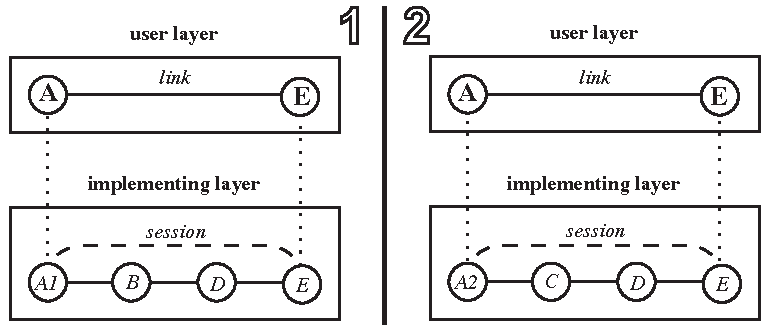
\includegraphics[scale=0.95]{figures/slm.pdf}
\caption{Two stages in an instance of session-location mobility.}
\label{fig:slm}
\end{figure}

This is a natural occurrence in a layer with a hierarchical name
space.
It should be 
familiar from observing what happens
when a laptop with an IP address {\it A1} moves to a new subnetwork
of the Internet, and gets a new IP address {\it A2} from DHCP.
The laptop cannot continue to use {\it A1} in the new subnetwork,
because {\it A1} is not in the subnetwork's address block.

DHCP alone is not sufficient to implement mobility, however.
As explained in Section~\ref{sec:layers.and.mobility}
and shown in Figure~\ref{fig:slm},
the strongest form of mobility requires preserving the 
communication channel in the user layer.
The bulk of the work of implementing session-location mobility lies in 
ensuring that {\bf A}'s correspondents know that it is now located at
{\it A2} rather than {\it A1}.
Each lower endpoint that was participating in a session with {\it A1}
on behalf of {\bf A} must be informed that it should now be corresponding
with {\it A2} instead.

As explained in Section~\ref{sec:layercomponents},
when an underlay is implementing a channel for an overlay, the initiating
lower endpoint must be able to look up the location of the 
accepting higher endpoint in the underlay, so that it can send messages
to it.
This means that there must be a globally accessible copy of the
{\it locations} mapping in the layer.
Session-location mobility also requires updating this mapping when
a higher endpoint moves.

Generally the fastest handoffs are achieved when a new lower endpoint
sends updates directly to all its correspondent lower endpoints
(in addition to updating the {\it locations} mapping).
This requires, of course, that the new lower endpoint have the 
correct name of the lower endpoint at the other end of each session.

Interesting behavior arises if both ends of a session move 
concurrently.
Neither lower endpoint will know the new name of the far endpoint,
so neither can send an update to the other.
In this simultaneous handoff
scenario a mobile endpoint, finding that it cannot reach a far
endpoint to update it, will suspect that the far endpoint has moved also.
Both endpoints must fall back on lookup from the {\it locations}
mapping to get the new location of the far endpoint.

As with Figure~\ref{fig:drm}, the two stages in Figure~\ref{fig:slm}
might have a gap between them or might overlap.
If they overlap, there will be an interval during which {\it A}
has two attachments in the same layer.

In Figure~\ref{fig:slm} the underlays are not shown,
although they probably look similar to those in Figure~\ref{fig:drm}.
Most likely there is an underlay member
{\it a1} that is destroyed, 
and an underlay member {\it a2} that is created.
There is no mobility observable at this level, however, because 
{\it A1} is attached to {\it a1} in Underlay 1 throughout its lifetime, and
{\it A2} is attached to {\it a2} in Underlay 2 throughout its lifetime.
The only mobility that is observable is {\bf A}'s change of attachment
from {\it A1} to {\it A2}.

Strictly speaking some dynamic routing could be involved in
session-location mobility, because
{\it A2} is a new member of the layer and there must be routes to it.
In practice this is rarely an issue, because the name
{\it A2} is part of some
larger block to which routes already exist.

Like DRM, session-location mobility (SLM) has storage costs,
update costs, and handoff latency.
The storage costs are the costs of maintaining a 
scalable implementation of {\it locations}.
The update costs are the costs of updating {\it locations} and
current correspondents when a member moves.

Implementations of SLM vary in a number of ways
(see Section~\ref{sec:sec6}),
although no one variation is as important as the hierarchical {\it versus}
non-hierarchical
variation for DRM.

\subsection{Major differences between the patterns}
\label{sec:majordifferences}

There are obvious structural differences between the two patterns:
\begin{itemize}
\item
In DRM the change of attachment appears between the implementing layer
and the level 
below it, while in SLM the change of attachment appears between
the user layer and the implementing layer 
(see Figures~\ref{fig:drm} and \ref{fig:slm}).
\item
In DRM the bulk of the work is performed by the routing algorithm,
while in SLM the bulk of the work is performed by the session protocol
and location algorithm (see Figure~\ref{fig:table}).
\item
In DRM the major state components that change are {\it attachments, links,}
and {\it routes} 
(see Figure~\ref{fig:table}).
In SLM the major state components that change are {\it locations}
and {\it sessions}. 
\end{itemize}
These structural differences prove that the two patterns are
fundamentally different.

In attempting to understand mobility mechanisms, people are sometimes
confused by the fact that {\it routes} (changed by DRM) and 
{\it locations} (changed by SLM) are both mappings.
The {\it locations} mapping is usually implemented by a shared global
data structure called a
{\it directory}.
The {\it routes} mapping is usually distributed across the forwarding
tables of the routers, but is occasionally implemented as a directory.
The result is that directories are sometimes used in both DRM and SLM
implementations.

This similarity is superficial because it does not tell
us the most important thing about
these mappings, which is what they mean in terms of
network architecture.
The mappings used in DRM and SLM are always fundamentally different, and
can always be distinguished from one another.
As mentioned in Section~\ref{sec:drm},
{\it routes} is a peer-to-peer or intra-layer mapping:
at each router, entries in the forwarding
table map each destination name to a member, link, or path {\it in the
same layer}. 
{\it Locations}, on the other hand, is always an inter-layer mapping,
mapping names in a higher layer to names in a lower layer.

In describing mobility mechanisms, people often focus on the
``identifier-locator split.''
This may be useful intuition, but should be interpreted carefully.
In an episode of mobility there is always a layer member that retains
its identity (the ``identifier''), and two members at a lower level,
where the attachment of the identifier moves from one to the other
(the ``locators'').
The identifier-locator split
does not distinguish DRM from SLM, although in the two patterns
the identifiers and locators appear at different levels.
In addition, it is important to remember that these terms are
relative, as mobility can occur anywhere in a layer hierarchy. 

On the surface, it may seem that DRM should be called ``in-network
mobility'' or the like, while SLM should be called ``end-to-end mobility''
or the like.
This reflects a misunderstanding of how general the patterns are,
and how freely they can be applied at different levels.
For one example, consider an application layer whose members run
only on Internet
hosts.
The members include user clients and named services.
The layer could have its own dynamic,
application-specific routing to services,
which allows services to be reached even though they move from server
to server.
This instance of DRM is not ``in network'' from most peoples' perspective.
For another example, an Internet router might itself be mobile,
and might have some of its links to other Internet routers
preserved as it moves by session-location
mobility at a lower level.
This instance of SLM does not involve any endpoints according to most
peoples' perspective.

Obviously a quantitative comparison between two mobility implementations
cannot be made without implementation details and a profile of the
expected load.
Nevertheless, it is possible to make some general comparisons
between the two patterns based on their potential strengths and 
weaknesses.
We say ``potential'' because any characteristic, whether positive or
negative, can be irrelevant in some situations.

The greatest potential
weakness of DRM is its storage, update, and path costs.
Normally routing information is different in different places,
so there is a lot of it, it is spread widely across a layer, and it
is expensive to update.
Attempts to economize on storage and update costs can lead to high
path costs (see Section~\ref{sec:sec5}), as messages travel further
to be routed successfully.
Path costs must be weighted heavily because {\it every}
message that travels on a
channel is affected by its path cost, if any.

Locations are very different from routes because the result of a location
query is usually the same no matter which member is querying (in
contrast to a route, which is different depending on where it is
starting from), and because a location query is needed only at the
beginning of a session and possibly after a move (in contrast to routes,
which are consulted on every hop of every message).
As a result, locations can be stored and updated much more cheaply
than routes.
For example, even a centralized directory would perform adequately
in many contexts.
And even if lookup of a location is slow, we do not count it as a
path cost because the cost is incurred a few times for each channel
rather than 
being built into the cost of transmitting each message on the channel.

The greatest potential
weakness of SLM is that it must be implemented with
the participation of session endpoints.
This means that deployment of an SLM mechanism requires new or
upgraded mobile devices that run the SLM protocol for sending and
receiving location updates.
Full interoperation with legacy endpoints calls for expensive middleboxes.
Security is a concern because endpoint devices can initiate
updates of the global layer state.

Concerns such as software upgrading and security have attracted less
attention with respect to DRM.
This is because a layer can, in principle, be designed so
that its members are partitioned into endpoints and routers, and
only the routers need be aware of or participate in an implementation
of DRM.
In reality these concerns are ubiquitous in distributed computing, and
can apply to routers as well.
